%%%%%%%%%%%%%%%%%%%%%%%%%%%%%%%%%%%%%%%%%%%%%%%%%%%%%%%%%%%%%%%%%%%%%%%%%%%%
% FILE    : Client.tex
% SUBJECT : Document describing design issues in the VTank Client.
% AUTHOR  : (C) Copyright 2009 by Vermont Technical College
%
%%%%%%%%%%%%%%%%%%%%%%%%%%%%%%%%%%%%%%%%%%%%%%%%%%%%%%%%%%%%%%%%%%%%%%%%%%%%

\chapter{\Client\ (client)}
\label{client}

\section{Requirements}

\Client\ is the name of the software that the user runs to play the \VTank\ game. The software uses Microsoft XNA Framework for .NET to render 3D models and textures to the screen, and Ice to communicate with \MainServer\ and \GameServer. From a regular user's perspective, the client is able to perform two functions:
\begin{itemize}
\item Manage the user's list of tanks.
\item Allow the user to play \VTank.
\end{itemize}

\subsection{Functional Requirements}

Once the client authenticates with the main server, it is allowed to perform some session-only actions. These actions include obtaining the user's personal list of tanks, requesting to join a game server, downloading a map, and other miscellaneous actions.

\Client\ uses Glacier2. This relieves users from having to open a port to play \VTank. 

\subsection{Use Cases}

The following case allows the user to authenticate with the main server.

\begin{usecase}
  {LOGIN}
  {Any User}
  {The client has just been opened and the user has not logged in yet.}
\begin{enumerate}
\item User enters account information into the 'Username' field.
\item User enters password into the 'Password' field.
\item A dialog box will appear informing the user that it is attempting to connect with the server. The user may press a 'Cancel' button to terminate the connection attempt.
\item If successful, the state of the client is changed to the tank selection screen.
\end{enumerate}
\end{usecase}

The following case allows a user to add a new tank to their list of tanks.

\begin{usecase}
  {ADDTANK}
  {Authenticated User}
  {The client has just logged in and is viewing his list of tanks.}
\begin{enumerate}
\item User has clicked the 'Add Tank' button.
\item User filled out forms about his new tank.
\item Data is sent through to the server, which will perform the updates. On error, a dialog box is presented.
\item If successful, the user is returned to the tank selection screen with the new tank present.
\end{enumerate}
\end{usecase}

The following case allows a user to modify an existing tank.

\begin{usecase}
  {EDITTANK}
  {Authenticated User}
  {The client has just logged in and is viewing his list of tanks.}
\begin{enumerate}
\item User has clicked the 'Edit Tank' button after highlighting a tank.
\item User edited fields regarding his tank.
\item Data is sent through to the server, which will perform the updates. On error, a dialog box is presented.
\item If successful, the user is returned to the tank selection screen with the modified tank present.
\end{enumerate}
\end{usecase}

The following case allows a user to delete an existing case.

\begin{usecase}
  {DELETETANK}
  {Authenticated User}
  {The client has just logged in and is viewing his list of tanks.}
\begin{enumerate}
\item User has clicked the 'Delete Tank' button after highlighting a tank.
\item Confirm dialog is presented to user: 'Cancel' returns, 'Confirm' proceeds.
\item Data is sent through to the server, which will perform the updates. On error, a dialog box is presented.
\item If successful, the user is returned to the tank selection screen with the tank removed.
\end{enumerate}
\end{usecase}

The following case allows a user to select which \GameServer\ to play on.

\begin{usecase}
	{SELECTSERVER}
	{Authenticated User}
	{The user selected his or her tank and is ready to play}
\begin{enumerate}
\item User has clicked the 'Game Server' button.
\item List of available servers are presented to the user.
\item The user highlights which server to join and then clicks the 'Join' button to proceed.
\item If successful, the state is changed to GamePlayState.
\end{enumerate}
\end{usecase}

The following case pulls up an in-game menu.

\begin{usecase}
	{INGAMEMENU}
	{Authenticated User}
	{The user is currently playing \Client.}
\begin{enumerate}
\item User hit the 'Escape' key during game play.
\item A Menu appears with the following options
	\begin{enumerate}
	\item \textbf{Resume} - Resume current game.
	\item \textbf{Options} - Brings up the Option menu that allows users to modify in-game options except video.
	\item \textbf{Log out} - Allows the user to log out and return to the Title screen.
	\item \textbf{Exit} - Exits \Client.
	\end{enumerate}
\item The user selects one of the option.
\end{enumerate}
\end{usecase}

\subsection{Install Script}

The install script will need to package up all of the necessary files required to run the VTank Client and make an executable installer that the user can run on their home machine. It will check for previous versions of DirectX and XNA and if they are not found or are outdated, it will install the required version. 

The installer will install the VTank Client in the Program Files folder by default, although the user may specify a different location if they wish. A shortcut should be placed on the desktop and in a start menu folder. The script should also create an uninstaller that will completely remove the VTank client from the user's PC (leaving DirectX and XNA intact) and place it in VTank's start menu folder. 

\subsection{Non-Functional Requirements}

\subsubsection*{Platform}

\Client\ alone can technically run on any XNA supported platform, which means the PC, XBox 360, and Zune. The client will only run on the PC currently. There are no plans to port \Client\ to the XBox 360 or the Zune, though it has been discussed. The issue with doing so is that Ice is not available for the .NET compact framework, which XBox 360 and Zune uses. If Ice were compiled for that platform, porting \Client\ to XBox 360 and Zune would be considered much more seriously.

\subsubsection*{Performance}

\Client's performance needs are a significant issue in programming, since poor code can result in horrible frame rate. \Client\ should be able to run on modern computers, and on modern operating systems at around 60 FPS without any issues.

\Client\ is rendered in 3D and this being the case, some modern computers may have difficulty running the client. It's important to detail minimum requirements as soon as possible. The minimum requirements should allow the user to run the software with reasonable frame rate no less than 30 FPS. 

The ability to tailor video option, such as the resolution, texture quality and anti-aliasing, on a user's machine can improve frame rate and performance.

\subsubsection*{Security}

The client must use IceSSL when first connecting to the server. Once it successfully authenticates with \MainServer, the client will start using the session and will no longer require SSL.

\Client\ has very little to do in terms of security. It should definitely do error checking to prevent it from bothering the server with obviously wrong information, yet clients cannot be trusted to give correct information. The server will always assume that the client is trying to sneak something bad in. It's the client's responsibility to be honest and to adhere to server demands (such as a demand to reset the tank's position to a ``legal'' one) -- otherwise the client will be kicked.

\subsubsection*{User Characteristics}

Users of \Client\ need to have no programming or development experience whatsoever. The client will be packaged in a way that makes it simple for users to download, install, update, reinstall, or uninstall \Client. Nothing more than minimum typing experience and some experience in gaming is required.

\subsubsection*{Scale}

The client more than any other software in the \VTank\ project will use a lot of memory. It must load in the map, a weapons database, an armor database, a projectile database, 3D models, textures, skins, audio clips, and much more. The most expensive objects will be the graphics, the audio, and (most significantly) the map. The user who creates maps should be careful not to upload maps that are too large.

\subsubsection*{Texture Naming Convention}

Each model has a texture mapped to it. To recognize what texture goes to which model, a naming convention is implemented. The naming convention follows the following format:  \texttt{[TextureModelName]\_texture.png}.

\subsubsection*{Data Formats}

When a new installer for a client is produced, a new ``local'' database is generated. The database is a XML file which is stored on the client-side. It works as a look-up table for what models should be used for certain types of objects. A XML-Linq library should be created to parse that file.

\subsubsection*{Internationalization}

\Client, more than any other software, has the opportunity for internationalization. If designed carefully from the beginning, error messages, dialog box text, labels, and everything else can be abstracted into a look-up table. The table has a section called ``English'', where all messages displayed in-game are stored. The user can be allowed to switch languages if needed.

\Client\ is currently only available in US English.

\section{Design and Architecture}

\Client\ makes use of several wrappers and libraries developed in house. The progression of the Client from startup to gameplay uses an approach much like a state machine. Each state performs a different task and then transitions to the next state. Each of these states is outlined in Figure~\ref{fig:clientUML}. 

\begin{figure}
	\centering
	\scalebox{0.5}{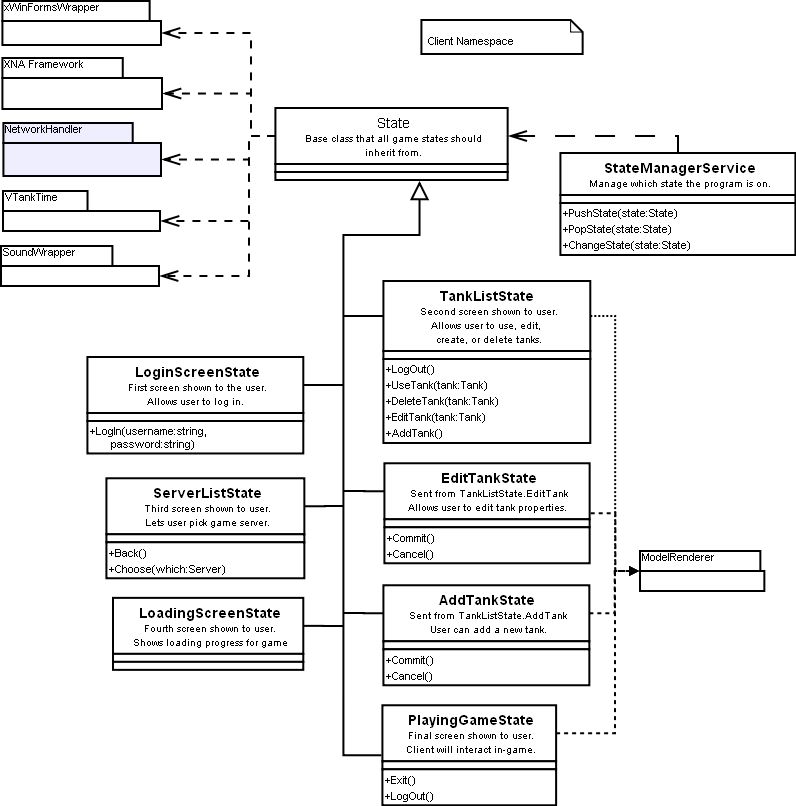
\includegraphics{Figures/Client.png}}
	\caption{\Client UML diagrams}
	\label{fig:clientUML}
\end{figure}

\begin{figure}
	\centering
	\scalebox{0.50}{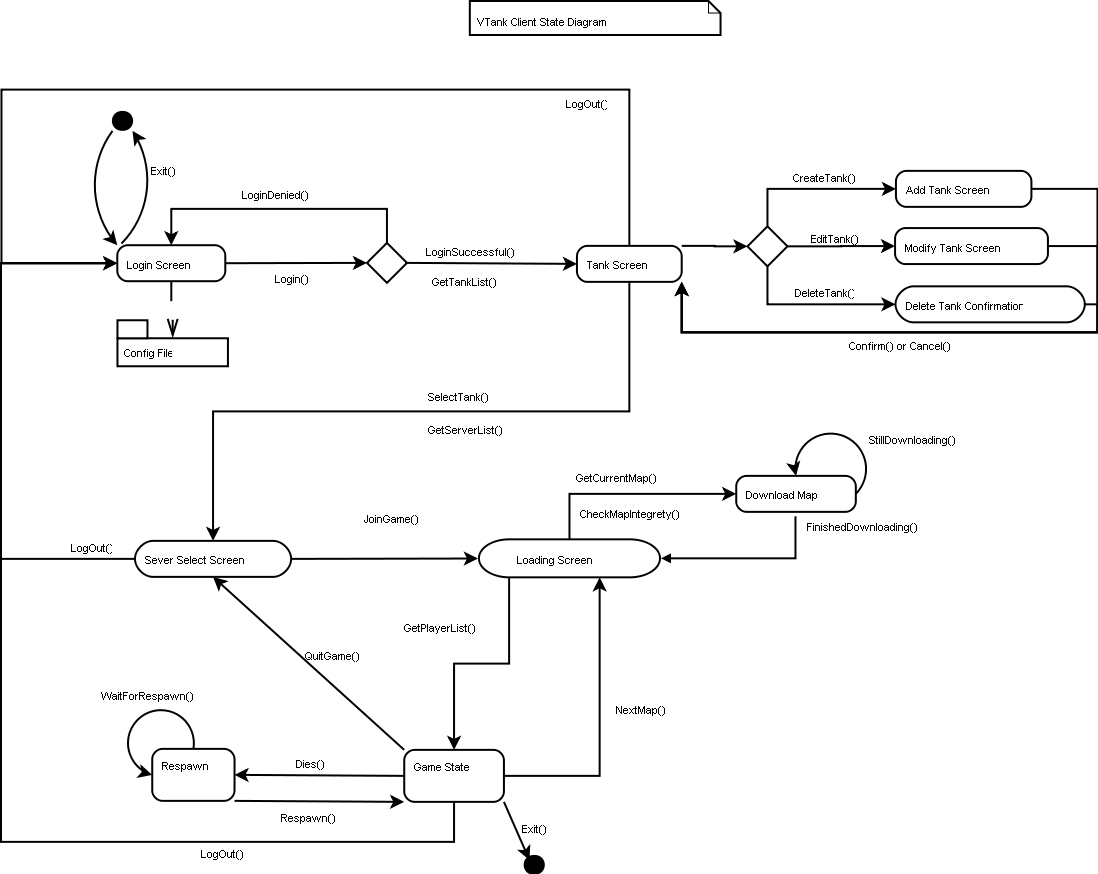
\includegraphics[angle=90]{Figures/ClientStateDiagram.png}}
	\caption{\Client\ state diagrams}
	\label{fig:clientstate}
\end{figure}

\subsection{Renderer}
Renderer is the tool that keeps track of and draws every model and sprite that is seen in the VTank game. Objects in Renderer are called \newterm{entities}. An entity can be a 3D Object, 2D Object, a camera or a light. They all use the same controls to move around in virtual space. Programmers make any object they want to insert into their game an extension of one of the entity classes and then Renderer will take care of moving, animating, and drawing them. 

\begin{center}
\begin{figure}
	\centering
		\scalebox{0.5}{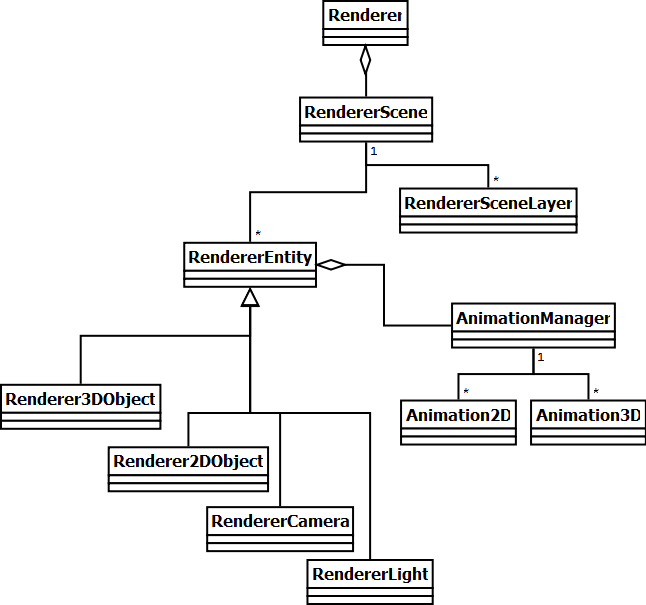
\includegraphics{UML/RendererClassDiagram.png}}
	\label{fig:Renderer Class Diagram}
\end{figure}
\end{center}

\subsection{VTank Networking}

This library will handle all the network operations for our client in a modular way. Such operations include but are not limited to: Connecting to the main server, connecting to a game server, sending a tank's actions, and keeping a connection alive.
  
\subsection{Audio Handler}

The audio handler will control all of the functions relating to storing and playing audio files in the game.

\section{Compiling}

This section assists in compiling \Client\ and all third party tools or libraries used.

\subsection{Windows}

\subsubsection{Building \Client}

\Client\ is a C\# project that uses XNA. Please download and install the following components:

\begin{itemize}
\item Visual Studio 2008 (alternatively, Visual C\# Express works too)
\item Microsoft XNA Framework v\XNAVersion
\item Ice v\IceVersion
\end{itemize}

Once installed, open the \Client\ solution (\filename{Client.sln}) file. Visual Studio will open the project. Build the project from here, and a fresh executable will be compiled.


\section{In-game Interface Components}

\subsection{HUD}

The HUD (Heads Up Display) is composed of two bars that wrap around the user's tank and convey to the user how much health they have and the remaining cooldown on their weapon, respectively.  In the case of special weapons, the cooldown bar may be replaced with a charge-up bar (blue), or an overheat bar (red) for certain weapons. These bars are customizable and scale with the resolution used by the player. It will also dynamically fade in and out based on whether it is being used. 

\begin{figure}[htbp]
	\centering
	\scalebox{0.50}{\includegraphics*{Figures/hud.png}}
	\caption{HUD}
	\label{fig:hud}
\end{figure}

\subsection{Minimap}

The VTank minimap shows a smaller version of what the user can currently see, but with a larger distance on all sides. It displays important information such as enemy/friend locations as well as map objectives such as flags and powerups. It will change to completely transparent if the user passes their mouse over it to avoid hiding an enemy behind it. 

\begin{figure}[htbp]
	\centering
	\scalebox{0.50}{\includegraphics*{Figures/minimap.png}}
	\caption{Minimap}
	\label{fig:mmap}
\end{figure}

\subsection{Scoreboard}

The VTank scoreboard will show the basic statistics for all players in the current game. It is updated in real time and will change formats based on the current type of game being played (DeathMatch, Capture the Flag, etc).  It also displays promotion and team round/game winning messages.

\begin{figure}[htbp]
	\centering
	\scalebox{0.50}{\includegraphics*{Figures/scoreboard.png}}
	\caption{Scoreboard}
	\label{fig:sboard}
\end{figure}

\subsection{Countdown Timer}

A countdown timer in the top left corner of the screen is used to inform players how long they have left before they respawn or when the map is going to change at the end of a game. 

\begin{figure}[htbp]
	\centering
	\scalebox{0.75}{\includegraphics*{Figures/timer.png}}
	\caption{Countdown timers for respawn and map change}
	\label{fig:timer}
\end{figure}

\subsection{\FormWrap Wrapper}

Figure~\ref{fig:formsWrapper}  shows how the client utilizes \FormWrap. A general purpose interface program is wrapped around front of the \FormWrap library to abstract out the creation of these forms. This way, another interface backend can be swapped in, and it will not be necessary to change the GameForm class. For the \FormWrap, the native focus and key/mouse handling support is somewhat lacking, so another layer was necessary to control these actions. The new layer will also be able to read in form configurations through a config files. This allows developers to modify the appearance of their GUI by either hand-modifying these files or through an external forms builder. 
 
\section{\Patcher}

\Patcher\ is the primary interface for the user to configure the client. By clicking the 'Options' button on \Patcher, the program spawns an external client configuration program. This program provides a user-friendly interface for modifying the client's config file, and provides options that affect video performance (resolution, anti-aliasing, fullscreen, refresh rate, quality, etc), audio performance (volume, mute), gameplay (profanity filter, interface options, etc), and input (re-mapping keys, cursor image).

\begin{figure}[htbp]
	\center
	\scalebox{0.75}{\includegraphics*{Figures/patcher.png}}
	\caption{Screenshot of \Patcher\ as of 08/09/2010.}
	\label{fig:launcher}
\end{figure}

Note that the patching functionality of the \Patcher\ is currently disabled.

\section{Particle Effects}

Particle effects are an integral part of the clients presentation method. A particle effect is currently defined by a particle emitter that contains a particle system. Both particle emitter and system can be loaded at runtime from .vtpes (VTank Particle Emitter Settings) and .vtpss (VTank Particle System Setting) files.

In VTank, these files are located in two folder, particleEmitterSettings and particleSystemSettings, that can be found under Client / Driver /Content / resources. To make a new emitter available in game, create a .vtpes and .vtpss file in the correct folders and add them to the Client project. Right click on all added particle files and select 'Properties'. Set 'Build Action' to 'None' and 'Copy to Output Directory' to 'Copy Always'. 
\begin{figure}[h]
	\centering
		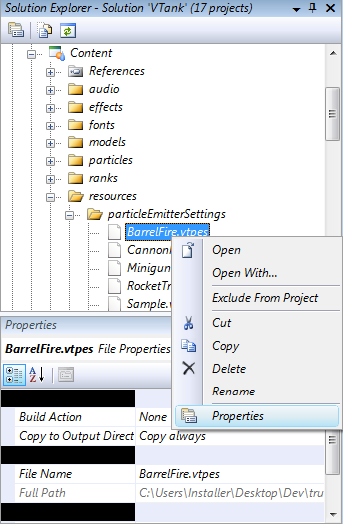
\includegraphics[width=0.50\textwidth]{Figures/AddParticleFiles.png}
	\label{fig:AddParticleFiles}
\end{figure}

Once you've done that the emitter will automatically be loaded into the RendererAssetPool and be available as an emitter. You can create the emitter by calling the ParticleEmitter constructor and passing the name of the file. For example, SuperEmitter.vtpes can be created with the following call:

ParticleEmitter newEmit = new ParticleEmitter("SuperEmitter");

Note that the parameters of a particle emitter setting object can be created dynamically. For example, to change the particle system assiciated with an emitter consider the following.

ParticleEmitterSettings setiings = RendererAssetPool.ParticleEmitterSettings["SuperEmitter"];
settings.ParticleSystemName = "differentSystemName";
ParticleEmitter pemit = new ParticleEmitter(settings);